\documentclass[12pt]{article}
\usepackage{amsmath}
\usepackage{graphicx,psfrag,epsf}
\usepackage{enumerate}
\usepackage{natbib}
\usepackage{url} % not crucial - just used below for the URL 

%\pdfminorversion=4
% NOTE: To produce blinded version, replace "0" with "1" below.
\newcommand{\blind}{0}

% DON'T change margins - should be 1 inch all around.
\addtolength{\oddsidemargin}{-.5in}%
\addtolength{\evensidemargin}{-.5in}%
\addtolength{\textwidth}{1in}%
\addtolength{\textheight}{1.3in}%
\addtolength{\topmargin}{-.8in}%


%%%% Packages and definitions
\usepackage{amssymb}

\usepackage{xr}
\externaldocument{hillclimbing_nonsmooth_appendix}

\usepackage[top=0.85in,left=1.0in,right=1.0in,footskip=0.75in]{geometry}

% Use adjustwidth environment to exceed column width (see example table in text)
\usepackage{changepage}

% Use Unicode characters when possible
\usepackage[utf8]{inputenc}

% textcomp package and marvosym package for additional characters
\usepackage{textcomp,marvosym}

\usepackage[ruled]{algorithm}
\usepackage{algorithmic}

% cite package, to clean up citations in the main text. Do not remove.
\usepackage{cite}

% Use nameref to cite supporting information files (see Supporting Information section for more info)
\usepackage{nameref,hyperref}

%\usepackage{amsthm}

% ligatures disabled
\usepackage{microtype}
\DisableLigatures[f]{encoding = *, family = * }

% for the beautiful checkmarks
\usepackage{pifont}

\newtheorem{theorem}{Theorem}
\newtheorem{definition}{Definition}
\newtheorem{condition}{Condition}

\DeclareMathOperator*{\argmin}{arg\,min}


\begin{document}

%\bibliographystyle{natbib}

\def\spacingset#1{\renewcommand{\baselinestretch}%
{#1}\small\normalsize} \spacingset{1}


%%%%%%%%%%%%%%%%%%%%%%%%%%%%%%%%%%%%%%%%%%%%%%%%%%%%%%%%%%%%%%%%%%%%%%%%%%%%%%

\if0\blind
{
  \title{\bf Gradient-based Regularization Parameter Selection for Problems with Non-smooth Penalty Functions}
  \author{Jean Feng\thanks{
    Jean Feng was supported by NIH grants DP5OD019820 and T32CA206089.
    Noah Simon was supported by NIH grant DP5OD019820.
    The content is solely the responsibility of the authors and does not necessarily represent the official views of the National Institutes of Health.}\\
    Department of Biostatistics, University of Washington\\
    and \\
    Noah Simon \\
    Department of Biostatistics, University of Washington}
  \maketitle
} \fi

\if1\blind
{
  \bigskip
  \bigskip
  \bigskip
  \begin{center}
    {\LARGE\bf Gradient-based Regularization Parameter Selection for Problems with Non-smooth Penalty Functions}
\end{center}
  \medskip
} \fi

\bigskip
\begin{abstract}
In high-dimensional and/or non-parametric regression problems, regularization (or penalization) is used to control model complexity and induce desired structure. Each penalty has a weight parameter that indicates how strongly the structure corresponding to that penalty should be enforced. Typically the parameters are chosen to minimize the error on a separate validation set using a simple grid search or a gradient-free optimization method. It is more efficient to tune parameters if the gradient can be determined, but this is often difficult for problems with non-smooth penalty functions. Here we show that for many penalized regression problems, the validation loss is actually smooth almost-everywhere with respect to the penalty parameters. We can therefore apply a modified gradient descent algorithm to tune parameters. Through simulation studies on example regression problems, we find that increasing the number of penalty parameters and tuning them using our method can decrease the generalization error.
\end{abstract}

\noindent%
{\it Keywords:}  cross-validation, high-dimensional regression, regularization, optimization
\vfill

\newpage
\spacingset{1.45} % DON'T change the spacing!
\section{Introduction}
Consider the usual regression framework with $p$ features, $\boldsymbol x_i = (x_{i1},\ldots,x_{ip})^\top$, and a response $y_i$ measured on each of $i=1,\ldots,n$ observations. Let $\boldsymbol X$ denote the $n \times p$ design matrix and $\boldsymbol y$ the response vector. Our goal here is to characterize the conditional relationship between $\boldsymbol y$ and $\boldsymbol X$. In simple low-dimensional problems this is often done by constructing an $f$ in some pre-specified class $\mathcal{F}$ that minimizes a measure of discrepancy between $\boldsymbol y$ and $f(\boldsymbol X)$. Generally, this discrepancy is quantified with some pre-specified loss, $L$. Often $\mathcal{F}$ will endow $f$ with some simple form (e.g. a linear function). For ill-posed or high-dimensional problems ($p \gg n$), there can often be an infinite number of solutions that minimize the loss function $L$ but have high generalization error. A common solution is to use regularization, or penalization, to select models with desirable properties, such as smoothness and sparsity.

In recent years, there has been much interest in combining regularization methods to produce models with multiple desired characteristics. Examples include the elastic net \citep{zou2003regression}, which combines the lasso and ridge penalties, and the sparse group lasso \citep{simon2013sparse}, which combines the group lasso and lasso penalties. The general form of these regression problems is:
\begin{equation} \label {eq:basic}
\hat f(\boldsymbol{\lambda}) = \argmin_{f\in\mathcal{F}} L\left (\boldsymbol{y}, f (\boldsymbol{X}) \right ) + \sum\limits_{i=1}^J \lambda_i P_i(f)
\end{equation}
where $\{P_i\}_{i=1, ..., J}$ are the penalty functions and $\boldsymbol{\lambda} = (\lambda_1, \ldots, \lambda_J)^\top$ are the regularization parameters. 

Regularization parameters control the degree of various facets of model complexity, such as the amount of sparsity or smoothness. Often the goal is to set the parameters to minimize the fitted model's generalization error. One usually estimates this using a training/validation approach (or cross validation). In this approach, one fits a model on a training set $(\boldsymbol X_T, \boldsymbol y_T)$ and measures the model's error on a validation set $(\boldsymbol X_V, \boldsymbol y_V)$. The goal then is to choose penalty parameters $\boldsymbol{\lambda}$ that minimize the validation error, as formulated in the following joint optimization problem:
\begin{equation}
\begin{array}{c}
\min_{\boldsymbol{\lambda} \in \Lambda} L\left (\boldsymbol{y}_V, \hat f (\boldsymbol{X}_V | \boldsymbol{\lambda}) \right) \\
\text{s.t. } \hat f(\cdot | \boldsymbol{\lambda}) = \argmin_{f\in\mathcal{F}} L \left (\boldsymbol{y}_T, f (\boldsymbol{X}_T) \right) + \sum\limits_{i=1}^J \lambda_i P_i(f)
\end{array}
\label{jointopt}
\end{equation}
Here $\Lambda$ is some set that $\boldsymbol{\lambda}$ are known to be in, which is often just $\mathbb{R}^{J}_+$. We will refer to finding $\hat f (\cdot | \boldsymbol{\lambda})$ as solving the inner optimization problem.

The simplest approach to solving \eqref{jointopt} is brute force: one fits models over a grid of parameter values and selects the model with the lowest validation error. As long as the grid is large and fine enough, this method of ``grid search" will find a solution close to the global optimum. Unfortunately, it is computationally intractable in cases with more than two parameters since the runtime is exponential in the number of parameters.

More efficient methods treat \eqref{jointopt} as a continuous optimization problem, usually through a gradient-free or gradient-based approach. Gradient-free approaches include the Nelder-Mead simplex algorithm \citep{nelder1965simplex} and Bayesian optimization \citep{snoek2012practical, bergstra2011algorithms, hutter2011sequential}. Although Bayesian optimization is currently the gold standard in machine learning, gradient-free methods are generally unable to tune more than twenty or so parameters whereas gradient-based methods can handle hundreds or even thousands of parameters. To calculate the gradient, one can use reverse-mode differentiation through the entire training procedure \citep{maclaurin2015gradient} or implicit differentiation of the KKT conditions \citep{larsen1998adaptive, bengio2000gradient, foo2008efficient, lorbert2010descent}. Existing implicit differentiation methods all require the optimization criterion to be smooth. In this paper we show that many problems for which the inner optimization problem is non-smooth can be reformulated in a way that makes them amenable to tuning parameter optimization via gradient descent.

In Section~\ref{defineDescJointOpt}, we show that for certain joint optimization problems with non-smooth penalties, the outer optimization problem is still smooth almost everywhere. By locally reformulating the problem, we can apply the same implicit differentiation trick to obtain the gradient of the validation loss with respect to the penalty parameters. A descent-based algorithm is then proposed for tuning the penalty parameters. Section~\ref{sec:results} presents three simulation studies comparing our method to gradient-free methods on regression problems with two to a hundred penalty parameters. We find that our method has lower generalization error compared to models trained with only two penalty parameters and outperforms gradient-free approaches. Section~\ref{realDataResults} applies our method to gene expression data to predict colitis status. The resulting models are significantly more sparse without sacrificing classification accuracy.

\section{Gradient-based Joint Optimization}\label{defineDescJointOpt}
\subsection{Definition}
In this manuscript we will restrict ourselves to classes $\mathcal{F} = \left\{f_{\boldsymbol \theta}\middle| \boldsymbol \theta\in\Theta\right\}$, which, for a fixed sample size $n$, are in some finite dimensional space $\Theta$. This is not a large restriction: the class of linear functions meets this requirement; as does any class of finite dimensional parametric functions. Even non-parametric methods generally either use a growing basis expansion (e.g. Polynomial regression, smoothing-splines, wavelet-based-regression, locally-adaptive regression splines \citep{tsybakov2008introduction, wahba1981spline, donoho1994ideal, mammen1997locally}), or only evaluate the function at the observed data-points (eg. trend filtering, fused lasso, \citep{kim2009ell_1, tibshirani2005sparsity}). In these non-parametric problems, for any fixed $n$, $\mathcal{F}$ is representable as a finite dimensional class.
We can therefore rewrite \eqref{eq:basic} in the following form:
\begin{equation}\label{eq:train_disc}
\argmin_{\boldsymbol \theta \in \Theta} L(\boldsymbol{y}, f_{\boldsymbol \theta}(\boldsymbol{X})) + \sum\limits_{i=1}^J \lambda_i P_i(\boldsymbol \theta)
\end{equation}

Suppose that we use a training/validation split to select penalty parameters $\boldsymbol{\lambda} = (\lambda_1, ..., \lambda_J)^\top$. Let the data be partitioned into a training set $(\boldsymbol{y}_T , \boldsymbol{X}_T)$ and validation set $(\boldsymbol{y}_V, \boldsymbol{X}_V)$. We can rewrite the joint optimization problem \eqref{jointopt} over this finite-dimensional class as:
\begin{equation}
\begin{array}{c}
\argmin_{\boldsymbol{\lambda} \in \Lambda} L(\boldsymbol{y}_V, f_{\hat{\boldsymbol \theta}(\boldsymbol{\lambda})}(\boldsymbol{X}_V)) \\
\text{s.t. } {\hat{\boldsymbol \theta}(\boldsymbol{\lambda})} = \argmin_{\boldsymbol \theta \in \Theta} L(\boldsymbol{y}_T, f_{\boldsymbol \theta} (\boldsymbol{X}_T)) + \sum\limits_{i=1}^J \lambda_i P_i(\boldsymbol \theta)
\end{array}
\label{jointopt2}
\end{equation}
Note that joint optimization for $K$-fold cross validation is very similar. The outer criterion is the average validation loss over the models trained from all $K$ folds. See the Appendix for the full formulation.

For the remainder of the manuscript we will assume that \eqref{eq:train_disc} for the training set is strictly convex in $\boldsymbol \theta$. This ensures that there is a unique $\hat{\boldsymbol \theta}(\boldsymbol{\lambda})$ which perturbs continuously in $\boldsymbol{\lambda}$. Also, we will assume that $L \left( \boldsymbol{y}_V, f_{\boldsymbol \theta}(\boldsymbol{X}_V) \right)$ is differentiable in $\boldsymbol \theta$. This assumption is met if both 1) $f_{\boldsymbol \theta}(\boldsymbol{X}_V)$ is continuous as a function of $\boldsymbol \theta$; and 2) $L\left(\boldsymbol{y}_V,\cdot\right)$ is smooth. Examples include the squared-error, logistic, and poisson loss functions, though not the hinge loss.

\subsection{Smooth Training Criterion}
Here we present a brief summary of the approach of applying gradient descent when the training criterion is smooth. For more details, refer to \citet{bengio2000gradient}.

Let the training criterion be denoted as
\begin{equation}
L_T\left(\boldsymbol \theta, \boldsymbol{\lambda}\right) \equiv L(\boldsymbol{y}_T, f_{\boldsymbol \theta} (\boldsymbol{X}_T)) + \sum\limits_{i=1}^J \lambda_i P_i(\boldsymbol \theta)
\label{train}
\end{equation}
To calculate the gradient, we apply the chain rule
\begin{equation}
\nabla_{\boldsymbol{\lambda}} L \left( \boldsymbol{y}_V, f_{\hat{\boldsymbol \theta}(\boldsymbol{\lambda})}(\boldsymbol{X}_V) \right ) = 
\left [
\left . \frac{\partial}{\partial \boldsymbol \theta} L ( \boldsymbol{y}_V, f_{\boldsymbol \theta}(\boldsymbol{X}_V)) \right |_{\boldsymbol \theta=\hat{\boldsymbol \theta}(\boldsymbol \lambda)}
\right ]^\top 
\frac{\partial}{\partial \boldsymbol{\lambda}} \hat{\boldsymbol \theta}(\boldsymbol{\lambda})
\label{chainrule}
\end{equation}
The first term, $\frac{\partial}{\partial \boldsymbol \theta} L ( \boldsymbol{y}_V, f_{\boldsymbol \theta}(\boldsymbol{X}_V))$, is problem specific, but generally straightforward to calculate. To calculate the second term, $\frac{\partial}{\partial \boldsymbol{\lambda}} \hat{\boldsymbol \theta}(\boldsymbol{\lambda})$, we note that $\hat{\boldsymbol \theta}(\boldsymbol{\lambda})$ minimizes \eqref{train}. Since \eqref{train} is smooth,
\begin{equation}
\nabla_\theta 
L_T(\boldsymbol \theta, \boldsymbol{\lambda})
|_{\boldsymbol \theta = \hat {\boldsymbol \theta}(\boldsymbol{\lambda})}
= \boldsymbol{0}.
\label{eq:grad}
\end{equation}
Taking the derivative of both sides of \eqref{eq:grad} in $\boldsymbol{\lambda}$ and solving for $\frac{\partial}{\partial \boldsymbol{\lambda}} \hat{\boldsymbol \theta}(\boldsymbol{\lambda})$, we get:
\begin{equation}
\frac{\partial}{\partial \boldsymbol{\lambda}} \hat{\boldsymbol \theta}(\boldsymbol{\lambda}) = 
- \left . \left [
 \nabla_\theta^2 L_T (\boldsymbol \theta, \boldsymbol{\lambda} )^{-1}
\nabla_{\boldsymbol \theta} P(\boldsymbol \theta)
\right ]
\right |_{\boldsymbol \theta = \hat {\boldsymbol \theta}(\boldsymbol{\lambda})}
\label{implicitDifferentiation}
\end{equation}
where $\nabla_{\boldsymbol \theta} P(\boldsymbol \theta)$ is the matrix with columns $\{\nabla_{\boldsymbol \theta} P_i(\boldsymbol \theta)\}_{i=1:J}$.

We can plug \eqref{implicitDifferentiation} into \eqref{chainrule} to get $\nabla_{\boldsymbol{\lambda}} L \left ( \boldsymbol{y}_V, f_{\hat{\boldsymbol \theta}(\boldsymbol{\lambda})}(\boldsymbol{X}_V) \right )$. Note that because $\frac{\partial}{\partial \boldsymbol{\lambda}} \hat{\boldsymbol \theta}(\boldsymbol{\lambda})$ is defined in terms of $\hat{\boldsymbol \theta}\left(\boldsymbol{\lambda}\right)$, each gradient step requires minimizing the training criterion first. The gradient descent algorithm to solve \eqref{jointopt2} is given in Algorithm \ref{alg:smooth}.

\begin{algorithm}
\caption{Gradient Descent for Smooth Training Criteria}
\label{alg:smooth}
\begin{algorithmic}
        \STATE{
	        	Initialize $\boldsymbol{\lambda}^{(0)}$.
	}
        \FOR{each iteration $k=0,1,...$ until stopping criteria is reached}
        \STATE{
        		Solve for $\hat {\boldsymbol \theta}(\boldsymbol{\lambda}^{(k)}) = \argmin_{\boldsymbol \theta \in \Theta} L_T(\boldsymbol \theta, \boldsymbol{\lambda}^{(k)})$.
	}
        \STATE{
        		Calculate the derivative of the model parameters with respect to the regularization parameters
                        	\begin{equation}
                        \frac{\partial}{\partial \boldsymbol{\lambda}} \hat{\boldsymbol \theta}(\boldsymbol{\lambda}) = 
                        - \left . \left [ \left (
                         \nabla_\theta^2 L_T(\boldsymbol \theta, \boldsymbol{\lambda}^{(k)})  \right )^{-1}
                        \nabla_{\boldsymbol \theta} P(\boldsymbol \theta)
                        \right ]
                        \right |_{\boldsymbol \theta = \hat {\boldsymbol \theta}(\boldsymbol{\lambda}^{(k)})}
                        \label{eq:gradient_hessian}
                        	\end{equation}
	}
	\STATE{
		Calculate the gradient
                      \begin{equation}
                      \left .
                      \nabla_{\boldsymbol{\lambda}} 
                      L \left (\boldsymbol{y_V}, f_{\hat {\boldsymbol \theta}(\boldsymbol{\lambda})}(\boldsymbol{X_V}) \right)
                      \right |_{\boldsymbol{\lambda} = \boldsymbol{\lambda}^{(k)}} =
                      \left [ \frac{\partial}{\partial \boldsymbol \theta} L(\boldsymbol{y}_V, f_{\boldsymbol \theta}(\boldsymbol{X_V})) \Big |_{\theta = \hat \theta(\boldsymbol{\lambda}^{(k)})} \right ]^\top
                      \frac{\partial}{\partial \boldsymbol{\lambda}} \hat{\boldsymbol \theta}(\boldsymbol{\lambda}) \Big |_{\boldsymbol{\lambda}=\boldsymbol{\lambda}^{(k)}}
                      \end{equation}
        }
        \STATE{Perform gradient step with step size $t^{(k)}$
	\begin{equation}
	\boldsymbol{\lambda}^{(k+1)} := \boldsymbol{\lambda}^{(k)} -
	t^{(k)}
	\left . \nabla_{\boldsymbol{\lambda}} L \left( \boldsymbol{y}_V, f_{\hat{\theta}(\boldsymbol{\lambda})}(\boldsymbol{X}_V)  \right )
	\right |_{\boldsymbol{\lambda} = \boldsymbol{\lambda}^{(k)}}
	\end{equation}
	}
	\ENDFOR
\end{algorithmic}
\end{algorithm}



\subsection{Nonsmooth Training Criterion}
When the penalized training criterion in the joint optimization problem is not smooth, gradient descent cannot be directly applied. Nonetheless, we find that in many problems, the solution $\hat{\boldsymbol \theta}\left(\boldsymbol{\lambda}\right)$ is smooth at almost every $\boldsymbol{\lambda}$ (eg. Lasso, Group Lasso, Trend Filtering); this means that we can indeed apply gradient descent in practice. In this section, we characterize these problems that are almost everywhere smooth. In addition, we provide a solution for deriving $\frac{\partial}{\partial \boldsymbol{\lambda}} \hat{\boldsymbol \theta}(\boldsymbol{\lambda})$ since calculating the gradient is a challenge in and of itself. This is then incorporated into an algorithm for tuning $\boldsymbol{\lambda}$ using gradient descent.

To characterize problems that are almost everywhere smooth, we begin with three definitions:
\begin{definition}
The differentiable space of a real-valued function $L$ at a point $\boldsymbol \eta$ in its domain is the set of vectors along which the directional derivative of $L$ exists.
\begin{equation}
\Omega^{L}(\boldsymbol \eta) = \left \{ \boldsymbol u \middle | \lim_{\epsilon \rightarrow 0} \frac{L(\boldsymbol \eta + \epsilon \boldsymbol u) - L(\boldsymbol \eta)}{\epsilon} \text{ exists } \right \}
\end{equation}
\end{definition}

\begin{definition}
$S$ is a local optimality space for a convex function $L(\cdot, \boldsymbol \lambda_0)$ if there exists a neighborhood $W$ containing $\boldsymbol \lambda_0$ such that for every $\boldsymbol \lambda \in W$,
\begin{equation}
\argmin_{\boldsymbol \theta \in \Theta} L(\boldsymbol \theta, \boldsymbol \lambda) =
\argmin_{\boldsymbol \theta \in S} L(\boldsymbol \theta, \boldsymbol \lambda)
\end{equation}
\end{definition}

\begin{definition}
Let matrix $\boldsymbol B = [ \boldsymbol b_1 \hdots \boldsymbol b_p ] \in \mathbb{R}^{n \times p}$ have orthonormal columns. Let $f$ be a real-valued function over $\mathbb{R}^n$ and suppose its first and second directional derivatives of $f$ with respect to the columns in $\boldsymbol B$ exist. The Gradient vector and Hessian matrix of $f$ with respect to $\boldsymbol B$ are defined respectively as
\begin{equation}\label{eq:hess}
_{\boldsymbol B} \nabla f  =
\left (
\begin{array}{c}
\frac{\partial f}{\partial \boldsymbol b_1} \\
\frac{\partial f}{\partial \boldsymbol b_2} \\
\vdots\\
\frac{\partial f}{\partial \boldsymbol b_p}\\
\end{array}
\right ) \in \mathbb{R}^p;
\quad
_{\boldsymbol B}\nabla^2 f =
\left (
\begin{array}{cccc}
\frac{\partial^2 f}{\partial b_1^2} & \frac{\partial^2 f}{\partial b_1 \partial b_2} & ...  & \frac{\partial^2 f}{\partial b_1 \partial b_p} \\
\frac{\partial^2 f}{\partial b_2 \partial b_1} & \frac{\partial^2 f}{\partial b_2^2} & ...  & \frac{\partial^2 f}{\partial b_2 \partial b_p} \\
\vdots & \vdots &  \ddots & \vdots \\
\frac{\partial^2 f}{\partial b_p \partial b_1} & \frac{\partial^2 f}{\partial b_p \partial b_2} & ...  & \frac{\partial^2 f}{\partial b_p^2} \\
\end{array}
\right ) \in \mathbb{R}^{p \times p}
\end{equation}
\end{definition}

Using these definitions we can now give three conditions which together are sufficient for the differentiability of $L \left( \boldsymbol{y}_V, f_{\hat{\boldsymbol \theta}(\boldsymbol{\lambda})}(\boldsymbol{X}_V) \right )$ almost everywhere.

\begin{condition}
For almost every $\boldsymbol{\lambda}$, the differentiable space $\Omega^{L_T(\cdot, \boldsymbol{\lambda})}(\hat{\boldsymbol \theta}\left(\boldsymbol{\lambda}\right))$ is a local optimality space for $L_T\left(\cdot,\boldsymbol{\lambda}\right)$.
\end{condition}

\begin{condition}
For almost every $\boldsymbol{\lambda}$, $L_T\left(\cdot, \cdot\right)$ restricted to $\Omega^{L_T(\cdot, \cdot)}(\hat{\boldsymbol \theta}\left(\boldsymbol{\lambda}\right), \boldsymbol{\lambda})$ is twice continuously differentiable within some neighborhood of $\boldsymbol{\lambda}$.
\end{condition}

\begin{condition}
For almost every $\boldsymbol{\lambda}$, there exists an orthonormal basis $\boldsymbol B$ of $\Omega^{L_T(\cdot, \boldsymbol{\lambda})}(\hat{\boldsymbol \theta}\left(\boldsymbol{\lambda}\right))$ such that the Hessian of $L_T\left(\cdot, \boldsymbol{\lambda}\right)$ at $\hat{\boldsymbol \theta}\left(\boldsymbol{\lambda}\right)$ with respect to $\boldsymbol B$ is invertible.

\end{condition}
Note that if condition 3 is satisfied, the Hessian of $L_T \left(\cdot, \boldsymbol{\lambda}\right)$ with respect to any orthonormal basis of $\Omega^{L_T(\cdot, \boldsymbol{\lambda})}(\hat{\boldsymbol \theta}\left(\boldsymbol{\lambda}\right))$ is invertible.

Putting all these conditions together, the following theorem establishes that the gradient exists almost everywhere and provides a recipe for calculating it.

\begin{theorem}
Suppose our optimization problem is of the form in \eqref{jointopt2}, with $L_T\left(\boldsymbol \theta, \boldsymbol{\lambda}\right)$ defined as in \eqref{train}.

Suppose that $L \Big( \boldsymbol{y}_V, f_{\boldsymbol \theta}(\boldsymbol{X}_V)\Big)$ is continuously differentiable in $\boldsymbol \theta$, and conditions $1$, $2$, and $3$, defined above, hold.

Then the validation loss $L(\boldsymbol{y_V}, f_{\hat {\boldsymbol\theta}(\boldsymbol{\lambda})}(\boldsymbol{X_V}))$ is continuously differentiable with respect to $\boldsymbol{\lambda}$ for almost every $\boldsymbol{\lambda}$. Furthermore, the gradient of $L(\boldsymbol{y_V}, f_{\hat \theta(\boldsymbol{\lambda})}(\boldsymbol{X_V}))$, where it is defined, is
\begin{equation}
\nabla_{\boldsymbol{\lambda}} L \left ( \boldsymbol{y_V}, f_{\hat {\boldsymbol \theta}(\boldsymbol{\lambda})}(\boldsymbol{X_V}) \right) =
\left [ \left .
\frac{\partial}{\partial \boldsymbol \theta} L(\boldsymbol{y_V}, f_{\boldsymbol \theta}(\boldsymbol{X_V}))
\right |_{\boldsymbol \theta=\tilde{\boldsymbol \theta}(\boldsymbol \lambda)} \right ]^\top
\frac{\partial}{\partial \boldsymbol{\lambda}} \tilde{\boldsymbol \theta}(\boldsymbol{\lambda})
\end{equation}
where
\begin{equation}
\tilde{\boldsymbol \theta}(\boldsymbol{\lambda}) = \argmin_{\boldsymbol \theta \in \Omega^{L_T(\cdot, \boldsymbol{\lambda})}(\hat {\boldsymbol \theta}(\boldsymbol{\lambda}))} L_T(\boldsymbol \theta , \boldsymbol{\lambda})
\label{restrictedmodelparams}
\end{equation}
\label{thethrm}
\end{theorem}

We can therefore construct a gradient descent procedure based on the model parameter constraint in \eqref{restrictedmodelparams}. At each iteration, let matrix $\boldsymbol U$ have orthonormal columns spanning the differentiable space $\Omega^{L_T(\cdot, \boldsymbol{\lambda})}(\hat {\boldsymbol \theta}(\boldsymbol{\lambda}))$. Since this space is also a local optimality space, it is sufficient to minimize the training criterion over the column space of $\boldsymbol U$. The joint optimization problem can be reformulated using $\boldsymbol U \hat {\boldsymbol \beta}(\boldsymbol{\lambda})$ as the model parameters instead:
\begin{equation}
\begin{array}{c}
\min_{\boldsymbol \lambda \in \Lambda} L(\boldsymbol y_V, f_{\boldsymbol U \hat{\boldsymbol \beta} (\boldsymbol \lambda) }(\boldsymbol X_V)) \\
\text{s.t. } \hat{\boldsymbol \beta} (\boldsymbol \lambda) =
\argmin_{\boldsymbol \beta}
L_T (\boldsymbol U \boldsymbol \beta, \boldsymbol{\lambda} )
\end{array}
\end{equation}

This locally equivalent problem now reduces to the simple case where the training criterion is smooth. As mentioned previously, implicit differentiation on the gradient condition then gives us $\frac{\partial}{\partial \boldsymbol \lambda}\hat{\boldsymbol \beta}(\boldsymbol \lambda)$, which gives us the value of interest
\begin{equation}
\frac{\partial}{\partial \boldsymbol \lambda}
\hat{\boldsymbol \theta}(\boldsymbol \lambda) =
\boldsymbol U
\frac{\partial}{\partial \boldsymbol \lambda}\hat{\boldsymbol \beta}(\boldsymbol \lambda)
\end{equation}
Note that because the differentiable space is a local optimality space and is thus locally constant, we can treat $\boldsymbol U$ as a constant in the gradient derivations. Algorithm~\ref{alg:gradDescent} provides the exact steps for tuning the regularization parameters.

\begin{algorithm}
\caption{\label{alg:gradDescent} Gradient-based Joint Optimization}
  \begin{algorithmic}
        \STATE{
        		Initialize $\boldsymbol{\lambda}^{(0)}$.
	}
        \FOR { each iteration $k=0,1,...$ until stopping criteria is reached}
		\STATE{
              		Solve for $\hat {\boldsymbol \theta}(\boldsymbol{\lambda}^{(k)}) = \argmin_{\theta \in \Theta} L_T(\boldsymbol \theta, \boldsymbol{\lambda}^{(k)})$.
		}
              	\STATE{
			Construct matrix $\boldsymbol U^{(k)}$, an orthonormal basis of $\Omega^{L_T(\cdot, \boldsymbol{\lambda})}\left (\hat{\boldsymbol \theta}(\boldsymbol{\lambda}^{(k)}) \right )$.
		}
              	\STATE{
			Define the locally equivalent joint optimization problem
                            \begin{equation*}
                            \begin{array}{c}
                            \min_{\boldsymbol \lambda \in \Lambda} L(\boldsymbol y_V, f_{\boldsymbol U^{(k)} \hat{\boldsymbol \beta} (\boldsymbol \lambda) }(\boldsymbol X_V)) \\
                            \text{s.t. } \hat{\boldsymbol \beta} (\boldsymbol \lambda) =
                            \argmin_{\boldsymbol \beta}
                            L_T (\boldsymbol U^{(k)}\boldsymbol \beta, \boldsymbol{\lambda} )
                            \end{array}
                            \end{equation*}
		}              
              	\STATE{
			Calculate $\frac{\partial}{\partial \boldsymbol \lambda} \hat{\boldsymbol \beta}(\boldsymbol{\lambda})|_{\boldsymbol{\lambda} = \boldsymbol{\lambda}^{(k)}}$ where 
                               \begin{equation*}
                               \frac{\partial}{\partial \boldsymbol \lambda} \hat{\boldsymbol \beta}(\boldsymbol{\lambda}) =
                    		-  \left . \left[
				\left (
                    		_{\boldsymbol U^{(k)}}\nabla^2 L_T (\boldsymbol U^{(k)}\boldsymbol \beta, \boldsymbol{\lambda} )
                    		\right )^{-1}
                    		{}_{\boldsymbol U^{(k)}}\nabla P(\boldsymbol U^{(k)}\boldsymbol \beta)
				\right ]
                    		\right |_{\boldsymbol \beta =  \hat{\boldsymbol \beta}(\boldsymbol \lambda)}
                               \end{equation*}
			with $_{\boldsymbol U^{(k)}}\nabla^2$ and $_{\boldsymbol U^{(k)}}\nabla$ are as defined in \eqref{eq:hess}.
		}
              
              	\STATE{
			Calculate the gradient $\nabla_{\boldsymbol{\lambda}} L(\boldsymbol{y_V}, f_{\hat \theta(\boldsymbol{\lambda})}(\boldsymbol{X_V})) |_{\boldsymbol{\lambda} = \boldsymbol{\lambda}^{(k)}}$ where
                                 \begin{equation*}
                                 \nabla_{\boldsymbol{\lambda}} L \left (\boldsymbol{y_V}, f_{\hat \theta(\boldsymbol{\lambda})}(\boldsymbol{X_V}) \right ) =
                    		\left [
                    	  	\boldsymbol U^{(k)}
                    		\frac{\partial}{\partial \boldsymbol \lambda} \hat{\boldsymbol \beta}(\boldsymbol{\lambda})
                    		\right ]^\top
                    		\left [ \left .
                    		_{\boldsymbol U^{(k)}}\nabla L\left (\boldsymbol{y_V}, f_{\boldsymbol U^{(k)}\boldsymbol \beta}(\boldsymbol{X_V}) \right )
                                   	\right |_{\boldsymbol \beta = \hat{\boldsymbol \beta}(\boldsymbol \lambda)}
                    		\right ]
                                 \end{equation*}
		}
              \STATE{
              		Perform the gradient update with step size $t^{(k)}$
                            	\begin{equation*}
                            	\boldsymbol{\lambda}^{(k+1)} :=
                            	\boldsymbol{\lambda}^{(k)} - t^{(k)}
                            	\left .
                            	\nabla_{\boldsymbol{\lambda}} L \left (\boldsymbol{y_V}, f_{\hat \theta(\boldsymbol{\lambda})}(\boldsymbol{X_V}) \right )
                            	\right |_{\boldsymbol{\lambda} = \boldsymbol{\lambda}^{(k)}}
                            	\end{equation*}
		}
	\ENDFOR
  \end{algorithmic}
\end{algorithm}

\subsection{Examples}\label{sec:examples}

To better understand the proposed gradient descent procedure, we present example joint optimization problems with nonsmooth criteria and their corresponding gradient calculations.

For ease of notation, we will let $S_{\boldsymbol{\lambda}}$ denote the differentiable space of $L_T(\cdot, \boldsymbol{\lambda})$ at $\hat{\boldsymbol{\theta}}(\boldsymbol{\lambda})$. All the example regressions satisfy the conditions in Theorem~\ref{thethrm}; details are included in the Appendix. Note that in some examples below, we add a ridge penalty with a fixed small coefficient $\epsilon > 0$ to ensure that the training criterion is strictly convex.

\subsubsection{Elastic Net}\label{sec:enet}

The elastic net \citep{zou2003regression} is a linear combination of the lasso and ridge penalties that encourages both sparsity and grouping of predictors. We tune the regularization parameters $\boldsymbol{\lambda} = (\lambda_1, \lambda_2)^\top$ according to the joint optimization problem:
\begin{equation}
\begin{array}{c}
\min_{\boldsymbol{\lambda} \in \mathbb{R}^2_{+}} \frac{1}{2} \| \boldsymbol{y}_V - \boldsymbol{X}_V \hat{\boldsymbol{\theta}} (\boldsymbol \lambda) \| ^2 \\
\text{s.t. }
\hat{\boldsymbol{\theta}} (\boldsymbol{\lambda}) = \argmin_{\boldsymbol{\theta}} \frac{1}{2} \| \boldsymbol{y}_T - \boldsymbol{X}_T \boldsymbol{\theta} \| ^2
+ \lambda_1 \| \boldsymbol{\theta} \|_1
+ \frac{1}{2}\lambda_2 \| \boldsymbol{\theta} \|_2^2
\end{array}
\end{equation}

The first step to finding the gradient is determining the differentiable space. Let the nonzero indices of $\hat{\boldsymbol{\theta}}(\boldsymbol{\lambda})$ be denoted $I(\boldsymbol\lambda) = \{i | \hat{\theta}_i(\boldsymbol\lambda) \ne 0 \text{ for } i=1,...,p \}$ and let $\boldsymbol I_{I(\boldsymbol \lambda)}$ be a submatrix of the identity matrix with columns $I(\boldsymbol\lambda)$. Since $|\cdot|$ is not differentiable at zero, the directional derivatives of $||\boldsymbol \theta||_1$ only exist along directions spanned by the columns of $\boldsymbol I_{I(\boldsymbol \lambda)}$. Thus the differentiable space at $\boldsymbol \lambda$ is $S_{\boldsymbol{\lambda}} = span(\boldsymbol I_{I(\boldsymbol \lambda)})$.

Let $\boldsymbol{X}_{T, I(\boldsymbol\lambda)} = \boldsymbol{X}_T \boldsymbol{I}_{I(\boldsymbol \lambda)}$ and $\boldsymbol{X}_{V, I(\boldsymbol\lambda)}  = \boldsymbol{X}_V \boldsymbol{I}_{I(\boldsymbol \lambda)}$.  The locally equivalent joint optimization problem is
\begin{equation}
\begin{array}{c}
\min_{\boldsymbol{\lambda} \in \mathbb{R}^2_{+}} \frac{1}{2} \| \boldsymbol{y}_V - \boldsymbol{X}_{V, I(\boldsymbol \lambda)} \hat{\boldsymbol{\beta}} (\boldsymbol \lambda) \| ^2 \\
\text{s.t. }
\hat{\boldsymbol{\beta}} (\boldsymbol{\lambda}) = \argmin_{\boldsymbol \beta} \frac{1}{2} \| \boldsymbol{y}_T - \boldsymbol{X}_{T, I(\boldsymbol \lambda)} \boldsymbol \beta \| ^2
+ \lambda_1 \| \boldsymbol \beta \|_1
+ \frac{1}{2}\lambda_2 \| \boldsymbol \beta \|_2^2
\end{array}
\end{equation}

Since the problem is now smooth, we can apply the chain rule to get the gradient of the validation loss
\begin{equation}
\nabla_{\boldsymbol \lambda} L(\boldsymbol{y_V}, f_{\hat{\boldsymbol{\theta}}(\lambda)}(\boldsymbol{X_V})) =
- \left (
\boldsymbol{X}_{V, I(\boldsymbol\lambda)}
\frac{\partial}{\partial \boldsymbol \lambda} \hat{\boldsymbol{\beta}}(\boldsymbol{\lambda})
\right )^{\top}
\left (
\boldsymbol y_V - \boldsymbol{X}_{V, I(\boldsymbol\lambda)} \hat{\boldsymbol{\beta}} (\boldsymbol{\lambda})
\right )
\end{equation}

and by \eqref{implicitDifferentiation},
\begin{equation}
\frac{\partial}{\partial \boldsymbol \lambda} \hat{\boldsymbol{\beta}}(\boldsymbol{\lambda}) = 
- \left ( 
\boldsymbol{X}_{T, I(\boldsymbol\lambda)}^\top \boldsymbol{X}_{T, I(\boldsymbol\lambda)} + \lambda_2 \boldsymbol{I}
\right )^{-1}
\begin{bmatrix}
sgn \left (\hat{\boldsymbol{\beta}} (\boldsymbol{\lambda}) \right ) &
\hat{\boldsymbol{\beta}} (\boldsymbol{\lambda})
\end{bmatrix}
\end{equation}

\subsubsection{Additive Models with Sparsity and Smoothness Penalties}\label{sec:additive}

Now consider the nonparametric regression problem given response $y$ and covariates $\boldsymbol{x} \in \mathbb{R}^p$. We suppose $y$ is the sum of $p$ univariate functions:
\begin{equation}
y = \sum_{i=1}^p f_i(x_i) + \epsilon
\end{equation}
Let $\boldsymbol{\theta}^{(i)} \equiv (f_i(x_{i1}), ..., f_i(x_{in}))$ be estimates of functions $f_i$ at the observations. The model is fit using the least squares loss with sparsity and smoothness penalties. More specifically, for each estimate $\boldsymbol{\theta}^{(i)}$, we add a group lasso penalty $\| \cdot \|_2$ to encourage sparsity at the function level and a lasso penalty on the second-order discrete differences to encourage smooth function estimates. Hence there are a total of $2p$ non-smooth functions in the training criterion.

This regression problem usually employs two regularization parameters, one for the sum of the sparsity penalties and one for the sum of the smoothness penalties \citep{buhlmann2011statistics}. In the joint optimization problem below, we use a separate penalty parameter for each of the smoothness penalties, resulting in a total of $p+1$ penalty parameters. Ideally the parameters could be tuned such that functions with nearly constant slope have large penalty parameters and ``wiggly" functions have small penalty parameters.

Define matrices $\boldsymbol{I}_T$ and $\boldsymbol{I}_V$ such that $\boldsymbol I_T \boldsymbol{\theta}^{(i)}$ and $\boldsymbol I_V \boldsymbol{\theta}^{(i)}$ are estimates for $f_i$ at the training and validation inputs, respectively. The joint optimization problem is
\begin{equation}
\begin{array}{c}
\min_{\boldsymbol\lambda \in \mathbb{R}^{p+1}_{+}} \frac{1}{2|V|}
\left \|
\boldsymbol{y}_V
- \boldsymbol{I}_V \sum_{i=1}^p \hat{\boldsymbol{\theta}}^{(i)}(\boldsymbol{\lambda})
\right \|^2_2 \\
\text{s.t. }
\hat{\boldsymbol{\theta}}^{(i)}(\boldsymbol{\lambda}) =
\argmin_{\boldsymbol{\theta}}
\frac{1}{2} \left \|
\boldsymbol{y}_T
- \boldsymbol{I}_T \sum_{i=1}^p \boldsymbol{\theta}^{(i)} \right \|^2_2
+ \lambda_0 \sum_{i=1}^p \| \boldsymbol{\theta}^{(i)} \|_2 \\
+ \frac{1}{2} \sum_{i=1}^p \lambda_i \left \| \boldsymbol{D}^{(2)}_{\boldsymbol{x}_i} \boldsymbol{\theta}^{(i)} \right \|_1
+ \frac{1}{2} \epsilon \sum_{i=1}^p \| \boldsymbol{\theta}^{(i)} \|_2^2
\end{array}
\label{aplmProblem}
\end{equation}


The differentiable space is straightforward to determine for this problem, though requires bulky notation. Define $I_i(\lambda)$ for $i=1,...,p$ to be the indices along which smoothness penalty is not differentiable
\begin{equation}
I_i(\lambda) = \left \{j | \left (\boldsymbol{D}^{(2)}_{\boldsymbol{x}_i} \hat{\boldsymbol \theta}^{(i)}(\boldsymbol\lambda) \right )_j = 0 \text{ for } j=1,...,n \right \}
\end{equation}
and
\begin{equation}
J(\lambda) = \left \{ i | \hat{\boldsymbol \theta}^{(i)}(\boldsymbol\lambda) \ne \boldsymbol 0 \text{ for } i=1,...,p \right \}
\end{equation}
The group lasso penalty $\|\cdot\|_2$ is not differentiable in any direction at ${\bf 0}$ and is differentiable in all directions elsewhere. Then $S_{\boldsymbol \lambda} = span(\boldsymbol {U}^{(1)}) \oplus ... \oplus span(\boldsymbol {U}^{(p)}) $ where $\boldsymbol {U}^{(i)} = \boldsymbol{0}$ if $\hat{\boldsymbol \theta}^{(i)}(\boldsymbol\lambda) = \boldsymbol 0$ and $\boldsymbol {U}^{(i)}$ is an orthonormal basis of $\mathcal{N}(\boldsymbol{I}_{I_i(\lambda)}\boldsymbol{D}^{(2)}_{\boldsymbol{x}_i})$ otherwise.

Now we can define the locally equivalent joint optimization problem:
\begin{equation}
\begin{array}{c}
\min_{\boldsymbol{\lambda} \in \mathbb{R}^{p+1}_{+}}
\frac{1}{2|V|} \left \| \boldsymbol{y}_V
- \boldsymbol{I}_V \sum_{i\in J(\boldsymbol\lambda)} \boldsymbol {U}^{(i)} \hat{\boldsymbol{\beta}}^{(i)}(\boldsymbol{\lambda})
 \right \|^2_2 \\
\text{s.t. }
\hat{\boldsymbol{\beta}}^{(i)}(\boldsymbol{\lambda}) = \argmin_{\boldsymbol \beta}
\frac{1}{2n} \left \| \boldsymbol{y}_T
- \boldsymbol{I}_T \sum_{i\in J(\boldsymbol\lambda)} \boldsymbol {U}^{(i)} \hat{\boldsymbol{\beta}}^{(i)}(\boldsymbol{\lambda})
\right \|^2_2
+ \lambda_0 \sum_{i\in J(\boldsymbol\lambda)}  \| \boldsymbol {U}^{(i)} \boldsymbol{\beta}^{(i)} \|_2 \\
+ \frac{1}{2} \sum_{i\in J(\boldsymbol\lambda)} \lambda_i \left \| \boldsymbol{D}^{(2)}_{\boldsymbol{x}_i} \boldsymbol {U}^{(i)} \boldsymbol{\beta}^{(i)} \right \|_1
+ \frac{1}{2} \epsilon \sum_{i\in J(\boldsymbol\lambda)} \| \boldsymbol {U}^{(i)} \boldsymbol{\beta}^{(i)} \|_2^2
\end{array}
\end{equation}
From \eqref{implicitDifferentiation} and the chain rule, we get that the gradient of the validation loss is:
\begin{equation}
\nabla_{\boldsymbol \lambda} L(\boldsymbol{y_V}, f_{\hat{\boldsymbol{\theta}}(\boldsymbol{\lambda})}(\boldsymbol{X_V})) =
- \frac{1}{|V|}
\left (
\boldsymbol{I}_V \sum_{i\in J(\boldsymbol\lambda)}  \boldsymbol {U}^{(i)} \frac{\partial}{\partial \boldsymbol\lambda} \hat{\boldsymbol{\beta}}^{(i)}(\boldsymbol{\lambda})
\right )^\top
\left (
\boldsymbol{y}_V - \boldsymbol{I}_V \sum_{i\in J(\boldsymbol\lambda)} \boldsymbol {U}^{(i)} \hat{\boldsymbol{\beta}}^{(i)} (\boldsymbol\lambda)
\right )
\end{equation}
where
\begin{equation}
\frac{\partial}{\partial \lambda_i} 
\begin{bmatrix}
\hat{\boldsymbol{\beta}}^{1}(\boldsymbol{\lambda})\\
...\\
\hat{\boldsymbol{\beta}}^{|J(\boldsymbol{\lambda})|}(\boldsymbol{\lambda})\\
\end{bmatrix}
= 
\boldsymbol{H}(\boldsymbol\lambda)^{-1}
\begin{bmatrix}
\begin{bmatrix}
\frac{\hat{\boldsymbol{\beta}}^{(1)}(\boldsymbol \lambda)}{||\boldsymbol {U}^{(1)}  \hat{\boldsymbol{\beta}}^{(1)} (\boldsymbol \lambda)||_2}\\
...\\
\frac{\hat{\boldsymbol \beta}^{(M)} (\boldsymbol \lambda)}{||\boldsymbol {U}^{(p)}  \hat{\boldsymbol{\beta}}^{(p)}(\boldsymbol \lambda)||_2}\\
\end{bmatrix}
&
\boldsymbol C(\boldsymbol \beta( \boldsymbol \lambda))
\end{bmatrix}
\label{eq:additive_gradient}
\end{equation}

The Hessian $\boldsymbol{H}(\boldsymbol\lambda)$ and matrix $C(\boldsymbol \beta( \boldsymbol \lambda))$ are defined in the Appendix.

\subsubsection{Un-pooled Sparse Group Lasso}\label{sec:sgl}

The sparse group lasso is a linear regression problem that combines the $\|\cdot\|_2$ and $\|\cdot\|_1$ penalties \citep{simon2013sparse}. This method is well-suited for problems where features have a natural grouping, and only a few of the features from a few of the groups are thought to have an effect on response (e.g. genes in gene pathways). Here we consider a generalized version of sparse group lasso by considering individual penalty parameters for each group lasso penalty. This additional flexibility allows setting covariate and covariate group effects to zero by different thresholds. Hence ``un-pooled" sparse group lasso may be better at modeling covariate groups with very different distributions.

The problem setup is as follows. Given $M$ covariate groups, suppose $\boldsymbol{X}$ and $\boldsymbol \theta$ are partitioned into $\boldsymbol{X}^{(m)}$ and $\boldsymbol \theta^{(m)}$ for groups $m = 1, ... , M$. We are interested in finding the optimal regularization parameters $\boldsymbol{\lambda} = (\lambda_0, \lambda_1,..., \lambda_M)^\top$. The joint optimization problem is formulated as follows.
\begin{equation}
\begin{array}{c}
\min_{\boldsymbol{\lambda} \in \mathbb{R}^{M+1}_{+}} \frac{1}{2|V|}
\left \| \boldsymbol{y}_V - \boldsymbol{X}_V \hat{\boldsymbol{\theta}}(\boldsymbol{\lambda}) \right \|^2_2 \\
\text{s.t. }
\hat{\boldsymbol{\theta}}(\boldsymbol{\lambda}) =
\argmin_{\boldsymbol{\theta}} \frac{1}{2|T|} 
\left \| \boldsymbol{y}_T - \boldsymbol{X}_T \boldsymbol{\theta} \right \|^2_2
+ \lambda_0 \| \boldsymbol\theta \|_1
+ \sum_{m=1}^M  \lambda_m \| \boldsymbol\theta^{(m)} \|_2
+ \frac{1}{2} \epsilon \| \boldsymbol\theta \|_2^2
\end{array}
\label{eq:unpooled_sgl}
\end{equation}

By the same logic as before, the differentiable space $S_{\boldsymbol \lambda}$ is $span(\boldsymbol I_{I(\boldsymbol\lambda)})$ where $I(\boldsymbol\lambda) = \{i | \hat{\theta}_i(\boldsymbol\lambda) \ne 0 \text{ for } i=1,...,p \}$ are the nonzero indices of $\hat{\boldsymbol{\theta}}(\boldsymbol{\lambda})$. Therefore the locally equivalent joint optimization problem is
\begin{equation}
\begin{array}{c}
\min_{\boldsymbol{\lambda} \in \mathbb{R}^{M+1}_{+}} \frac{1}{2|V|} \left \| \boldsymbol{y}_V - \boldsymbol X_{V,I(\boldsymbol\lambda)} \hat{\boldsymbol\beta}(\boldsymbol{\lambda}) \right \|^2_2 \\
\text{s.t. }
\hat{\boldsymbol{\beta}}(\boldsymbol{\lambda}) = \argmin_{\boldsymbol \beta}
\frac{1}{2|T|} \left \| \boldsymbol{y}_T - \boldsymbol{X}_{T, I(\boldsymbol\lambda)} \boldsymbol \beta \right \|^2_2
+ \lambda_0 \| \boldsymbol \beta \|_1
+ \sum_{m=1}^M \lambda_m \| \boldsymbol \beta^{(m)} \|_2
+ \frac{1}{2}\epsilon \| \boldsymbol \beta \|_2^2
\end{array}
\end{equation}
where we use the same notational shorthand $\boldsymbol{X}_{T, I(\boldsymbol\lambda)}$ and $\boldsymbol{X}_{V, I(\boldsymbol\lambda)}$ from Section \ref{sec:enet}.

From \eqref{implicitDifferentiation} and the chain rule, we get that the gradient of the validation loss is
\begin{equation}
\nabla_{\boldsymbol \lambda} L(\boldsymbol{y_V}, f_{\hat{\boldsymbol{\theta}}(\boldsymbol{\lambda})}(\boldsymbol{X_V})) =
- \frac{1}{n}
\left (
\boldsymbol{X}_{V, I(\boldsymbol\lambda)}
\frac{\partial}{\partial \boldsymbol\lambda} \hat{\boldsymbol{\beta}}(\boldsymbol{\lambda})
\right )^\top
\left (
\boldsymbol{y}_V - \boldsymbol{X}_{V, I(\boldsymbol\lambda)} \hat{\boldsymbol{\beta}}(\boldsymbol{\lambda})
\right )
\end{equation}
where 
\begin{equation}
\frac{\partial}{\partial \boldsymbol \lambda} \hat{\boldsymbol{\beta}}(\boldsymbol{\lambda})
=
- \boldsymbol H(\boldsymbol \lambda)^{-1}
\begin{bmatrix}
\boldsymbol C(\hat{\boldsymbol \beta}(\boldsymbol \lambda)) & sgn(\hat {\boldsymbol \beta}(\boldsymbol \lambda))
\end{bmatrix}
\label{eq:unpooled_sgl_grad}
\end{equation}
The Hessian $\boldsymbol H(\boldsymbol \lambda)$ and the matrix $\boldsymbol C(\hat{\boldsymbol \beta}(\boldsymbol \lambda))$ are given in the Appendix.

\subsection{Gradient Descent Details}\label{sec:alg_details}
Here we discuss choice of step size and our convergence criterion.

There are many possible choices for our step size sequence $\{t^{(k)}\}$. Popular choices for convex problems are discussed in \citet{boyd2004convex}. We chose a backtracking line search as discussed in Chapter 9. In our examples initial step size was between 0.5 and 1 and we backtrack with parameters $\alpha \in [0.001, 0.01]$ and $\beta \in [0.01, 0.1]$. Details of backtracking line search are given in the Appendix. During gradient descent, it is possible that the step size will result in a negative regularization parameter; we reject any step that would set a regularization parameter to below a minimum threshold of $1e$-6.

Our convergence criterion is based on the change in our validation loss between iterates. More specifically, we stop our algorithm when
\[
L \left( \boldsymbol{y}_V, f_{\hat{\boldsymbol \theta}(\boldsymbol{\lambda}^{(k+1)})}(\boldsymbol{X}_V)\right) -
L \left( \boldsymbol{y}_V, f_{\hat{\boldsymbol \theta}(\boldsymbol{\lambda}^{(k)})}(\boldsymbol{X}_V)\right) \leq \delta
\]
for some prespecified tolerance $\delta$. For the results in this manuscript we use $\delta \in [0.05, 1e\text{-}4]$.

\section{Simulation Studies}\label{sec:results}

We now compare our gradient descent algorithm to gradient-free methods through simulation studies. Each simulation corresponds to a joint optimization problem given in Section \ref{sec:examples}. We tune the regularization parameters over a training/validation split using gradient descent, Nelder-Mead, and the Bayesian optimization solver from \citet{snoek2012practical} called Spearmint. For baseline comparison, we also solve a two-parameter version of the joint optimization problem using grid search.

We compare the efficiency of the methods by the number of times the methods solved the inner training criterion (labeled ``\# Solves" in the tables below). We set this number to 100 for all three gradient-free methods. This number is variable for gradient descent since it depends on how fast the algorithm converges.

% Inner training criteria were solved using the splitting conic solver (SCS) or ECOS in CVXPY \citep{cvxpy}, depending on the accuracy of the solver for the particular problem. Spearmint was allowed to solve the inner optimization problem at 100 penalty parameter points. Nelder-Mead was allowed fifty evaluations for each initialization point. Grid search was performed over a $10 \times 10$ log-spaced grid. To compare the efficiency of the methods, we provide the number of times gradient descent solved the inner optimization problem (labeled ``\# Solves"). 

There are two computational concerns when tuning regularization parameters by gradient descent. First, the gradient calculation can be slow if the matrix in \eqref{eq:gradient_hessian} is large. \citet{bengio2000gradient} and \citet{foo2008efficient} suggest backpropagating through a Cholesky decomposition or using conjugate gradients to speed this up. This is actually not an issue for problems with non-smooth training criteria since the solutions tend to be sparse, which result in small linear systems. The second concern is that the inner optimization problem must be solved to a high accuracy in order to calculate the gradient. (Recall that the gradient is derived via implicit differentiation.) To address this, we allow more iterations for solving the inner optimization problem. For a faster implementation of gradient descent, one can use a more specialized solver.

In each section below, we provide the simulation settings followed by a discussion of the results.

\subsection{Elastic Net}
Each dataset consists of 80 training and 20 validation observations with 250 predictors. The $\boldsymbol x_i$ were marginally distributed $N(\boldsymbol 0,\boldsymbol I)$ with $cor(x_{ij},x_{ik}) = 0.5^{|j-k|}$.
The response vector $\boldsymbol y$ was generated by
\begin{equation}
\boldsymbol y = \boldsymbol X \boldsymbol \beta + \sigma \boldsymbol \epsilon \; \text{where} \; \boldsymbol \beta = (\underbrace{1, ..., 1}_\text{size 15}, \underbrace{0, ..., 0}_\text{size 235})
\end{equation}
and $\boldsymbol \epsilon \sim N(\boldsymbol 0, \boldsymbol I)$. $\sigma$ was chosen such that the signal to noise ratio is 2. 

Grid search was performed over a $10 \times 10$ log-spaced grid from 1$e$-5 to 100. Nelder-mead and gradient descent were initialized at (0.01, 0.01) and (10, 10). Nelder-mead was allowed fifty iterations starting from each initialization point.

As shown in Table \ref{tab:elasticnet}, all the methods achieve similar validation errors. For this simple problem, the benefit for using gradient descent is not significant.

\begin{table}
\caption {\label{tab:elasticnet} Comparison of solvers for Elastic Net joint optimization problem}
\centering
\begin{tabular}{| l | l | l | }
\hline
& Validation Error & \# Solves\\
\hline
% (1122 + 494 - 148 - 389)/30
Gradient Descent & 5.20 (0.20) & 36.0 \\
\hline
Nelder-Mead & 5.11 (0.20) & 50 \\
\hline
Spearmint & 5.49 (0.22) & 100 \\
\hline
Grid Search & 5.22 (0.18) & 100 \\
\hline
\end{tabular}
\end{table}


\subsection{Additive model with Smoothness and Sparsity Penalty}
Each dataset consists of 150 training, 75 validation, and 75 test observations with $p=23$ covariates. The covariates $\boldsymbol{x_i} \in \mathbb{R}^{n}$ for $i=1,...p$ are equally spaced from -5 to 5 with a random displacement $ \delta \sim U(0, \frac{1}{300}) $ at the start and then shuffled randomly. The true model is the sum of three nonzero functions and 20 zero functions. Response $y$ was generated as follows
\begin{eqnarray*}
\boldsymbol y &=& \sum\limits_{i=1}^p \boldsymbol f_i(\boldsymbol x_i) + \sigma \boldsymbol \epsilon\\
f_1(x) &=& 9 \sin(3x)\\
f_2(x) &=& x\\
f_3(x) &=& 6 \cos(1.25 x) + 6 \sin(0.5 x + 0.5)\\
f_i(x) &=& 0 \text{ for }   i=4,...,23\\
\end{eqnarray*}
where $\boldsymbol \epsilon \sim N(\boldsymbol 0, \boldsymbol I)$. $\sigma$ was chosen such that the signal to noise ratio was 2.

Nelder-Mead and gradient descent were both initialized at $(10, 1, ..., 1)$ and $(0.1, 0.01, ..., 0.01)$. Nelder-mead was allowed fifty iterations starting from each initialization point.

For baseline comparison, we also solved a two-parameter version of this joint optimization problem by pooling $\{\lambda_i\}_{i=1:p}$ into a single $\lambda_1$. Grid search was then performed over a $10 \times 10$ log-spaced grid from 1$e$-4 to $100$. 

As shown in Table \ref{tab:additive}, gradient descent returned models with the lowest test error on average. We can see that the joint optimization problem with 24 penalty parameters is sensitive to the penalty parameters chosen; Spearmint returned a result that is not only worse than gradient descent but even worse than grid search over the pooled two-parameter joint optimization problem.

Table \ref{tab:additive_average_lambda} provides the average penalty parameter values for $\lambda_0, ..., \lambda_4$. Gradient descent was indeed able to determine the smoothness of the functions. It tended to choose $\lambda_1$ to have the smallest value and $\lambda_2$ to have the largest value, which corresponds to the fact that the slope for $f_1$ varies the most and the slope for $f_2$ is constant. In contrast, Nelder-Mead wasn't able to determine the difference in smoothness between the functions and kept all penalty parameters the same. Spearmint chose a very different set of parameters that don't seem to be appropriate for the problem.

Figure \ref{fig:additive} provides example model fits given by gradient descent. The smoothness of the function estimates reflect the magnitude of the regularization parameters given in Table \ref{tab:additive}. In addition, gradient descent was able to learn that $f_4$ was the zero function.

\begin{table}
\caption {\label{tab:additive} A comparison of additive models with separate smoothness penalty parameters tuned by gradient descent, Nelder-Mead, and Spearmint vs. additive models with two penalty parameters tuned by grid search. Standard errors are given in parentheses.}
\centering
\begin{tabular}{| l | l | l | l | l | }
\hline
& Num $\lambda$ & Validation Error & Test Error & \# Solves\\
\hline
% (729 + 351 - 87 - 184)/30
Gradient Descent & 24 & 23.91 (0.93) & 26.15 (0.78) & 27.0 \\
\hline
Nelder-Mead & 24 & 27.91 (0.90) & 28.73 (0.90) & 100 \\
\hline
Spearmint & 24 & 32.64 (2.03) & 37.72 (2.17) & 100 \\
\hline
Grid Search & 2 & 28.85 (0.92) & 30.03 (0.97) & 100 \\
\hline
\end{tabular}
\end{table}

\begin{table}
\caption {\label{tab:additive_average_lambda} Average $\lambda_i$ values for the fitted models}
\centering
\begin{tabular}{| l | l | l | l | l | l | }
\hline
& $\lambda_0$ & $\lambda_1$ & $\lambda_2$ & $\lambda_3$ & $\lambda_4$\\
\hline
Gradient Descent & 9.96 & 0.40 & 1.01 & 0.86 & 1.04 \\
\hline
Nelder-Mead & 9.69 & 0.90 & 1.01 & 1.00 & 1.00 \\
\hline
Spearmint & 3.36 & 0.76 & 0.06 & 0.01 & 0.03\\
\hline
Grid Search & 4.65 & 0.44 & -- & -- & -- \\
\hline
\end{tabular}
\end{table}

\begin{figure}
\caption{Example model fits given by gradient descent for $f_1, f_2, f_3,$ and $ f_4$. The dashed lines are the true functions and the solid lines are the estimated functions. (Top left: $f_1$, top right: $f_2$, bottom left: $f_3$, bottom right: $f_4$)}
\centering
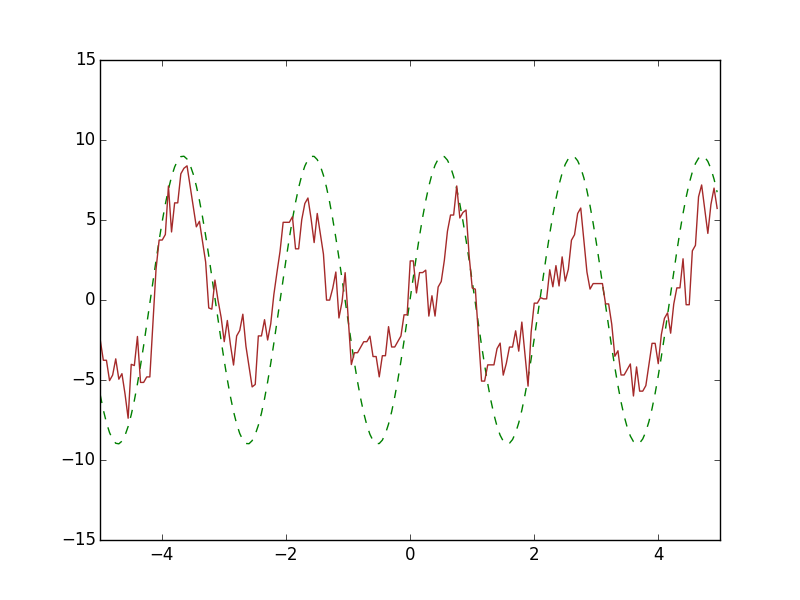
\includegraphics[height=50mm]{sparse_add_model_3_20_100_50_50_func0.png}
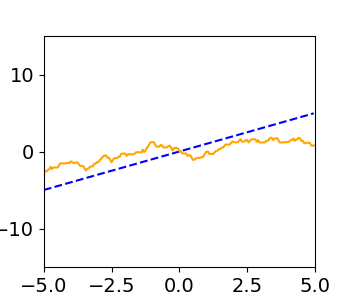
\includegraphics[height=50mm]{sparse_add_model_3_20_100_50_50_func1.png}
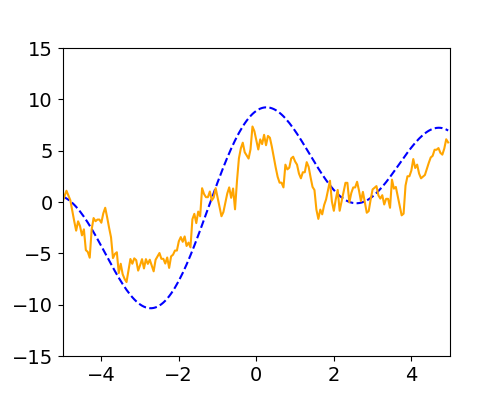
\includegraphics[height=50mm]{sparse_add_model_3_20_100_50_50_func2.png}
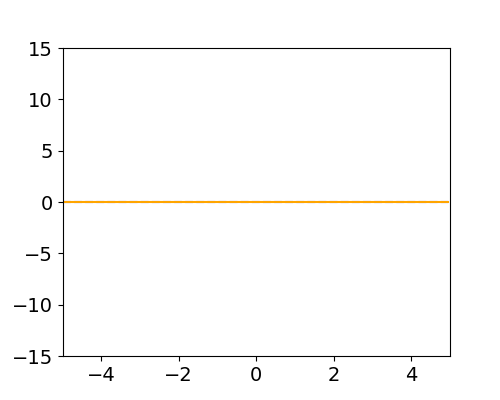
\includegraphics[height=50mm]{sparse_add_model_3_20_100_50_50_func3.png}
\label{fig:additive}
\end{figure}


\subsection{Sparse group lasso}\label{sec:simulation_sgl}
We ran three experiments with different numbers of covariate groups $M$ and total covariates $p$, as given in Table \ref{table:unpooled}. For each experiment, the dataset consisted of $n$ training, $n/3$ validation, and 200 test observations. The predictors $\boldsymbol X$ were generated from a standard normal distribution. The response $\boldsymbol y$ was generated by
\begin{equation}
\boldsymbol y = \sum\limits_{j=1}^3 \boldsymbol X^{(j)} \boldsymbol \beta^{(j)} + \sigma \boldsymbol \epsilon \; \text{where} \; \boldsymbol \beta^{(j)} = (1, 2, 3, 4, 5, 0, ..., 0)
\end{equation}
where $\boldsymbol \epsilon \sim N(\boldsymbol 0, \boldsymbol I)$. $\sigma$ was chosen such that the signal to noise ratio was 2. 

We compare gradient descent against all three gradient-free methods in the first experiment with 31 regularization parameters and only compare against grid search for the latter experiments with 61 and 101 regularization parameters. Gradient-free methods are generally not recommended for tuning more than thirty parameters; Spearmint's implementation is limited to no more than forty hyperparameters and Nelder-Mead performed poorly. For all experiments, grid search solved a two-parameter version where $\{\lambda_i\}_{i=1:M}$ are pooled into a single $\lambda_2$.

For all three experiments, grid search was performed over a $10 \times 10$ grid from 1$e$-3 to $10$. Gradient descent was initialized at $0.1 \times \boldsymbol 1$ and $\boldsymbol 1$. Nelder-Mead was initialized at the same points for the first experiment.

Model performance was assessed using three metrics: test error, $\beta$ error (defined as $\| \boldsymbol \beta - \hat {\boldsymbol \beta} \|_2$), and the percentage of nonzero coefficients correctly identified among all the true nonzero coefficients. As shown in Table \ref{table:unpooled}, the model tuned by gradient descent produced the lowest test error and $\beta$ error in all three experiments. Nelder-Mead struggled to minimize the validation error and the models were very similar to the models returned by grid search on the two-parameter problem. Interestingly, Spearmint found models with small validation error but they had the worst performance by the three metrics.

\begin{table}
\caption{\label{table:unpooled} Un-pooled sparse group lasso and sparse group lasso (SGL) tuned by gradient descent and grid search, respectively. ``\% CN $\beta$" is the percentage of nonzero coefficients correctly identified among all the true nonzero coefficients. Standard errors are given in parentheses.}
\centering
\begin{tabular}{| l | l | l | l | l | l | l |}
\hline
\multicolumn{7}{|c|}{n=60, p=300, g=3, M=30}\\
\hline
& \# $\lambda$ & $\beta$ Error & \% CN $\beta$ & Validation Err & Test Err & \# Solves \\
\hline
% 292 + 598 iters, 746 + 1518 CVX solves, (746 + 1518 - (292 + 598))/30 total solves
Gradient Descent & 31 & 7.27 (0.30) & 87.78 (2.04) & 22.56 (1.72) & 47.55 (3.00) & 45.8 \\
\hline
Nelder-Mead & 31 & 8.44 (0.22) & 75.11 (2.01) & 57.27 (4.02) & 56.57 (1.98) & 100\\
\hline
Spearmint & 31 & 8.91 (0.32) & 78.89 (2.46) & 28.25 (2.56) & 60.60 (2.98) & 100\\
\hline
Grid search & 2 & 8.50 (0.25) & 83.78 (2.57) & 52.32 (3.66) & 56.86 (2.10) & 100 \\
\hline
\multicolumn{7}{|c|}{n=90, p=900, g=3, M=60}\\
\hline
& \# $\lambda$ & $\beta$ Error & \% CN $\beta$ & Validation Error & Test Error & \# Solves \\
\hline
% 578 + 344 iters, 1479 + 848 solves
Gradient Descent & 61 & 6.35 (0.20) & 90.00 (1.60) & 18.40 (1.21) & 41.48 (1.40) & 46.83 \\
\hline
Grid Search & 2 & 7.67 (0.20) & 84.67 (1.97) & 45.70 (2.27) & 51.34 (1.86) & 100 \\
\hline
\multicolumn{7}{|c|}{n=90, p=1200, g=3, M=100}\\
\hline
& \# $\lambda$ & $\beta$ Error & \% CN $\beta$ & Validation Error & Test Error & \# Solves \\
\hline
%  iters 599 + 371, 1524 + 889 solves
Gradient Descent & 101 & 6.82 (0.25) & 89.78 (1.80) & 18.43 (1.42) & 46.36 (1.94) & 48.1 \\
\hline
Grid Search & 2 & 8.28 (0.19) & 86.00 (1.97) & 50.00 (2.16) & 57.14 (2.18) & 100 \\
\hline
\end{tabular}
\end{table}


\section{Application to Biological Data}\label{realDataResults}
Finally, we applied our algorithm in a real data example. More specifically, we considered the problem of finding predictive genes from gene pathways for Crohn's Disease and Ulcerative Colitis. \citet{simon2013sparse} addressed this problem using the sparse group lasso; we now compare this against applying the un-pooled sparse group lasso, where the regularization parameters were tuned using gradient descent. Since this is a classification task, the joint optimization problem is the same as \eqref{eq:unpooled_sgl} but with the logistic loss:
\begin{equation}
L\left ( \boldsymbol{y}, f_{\boldsymbol \beta(\boldsymbol\lambda)}(\boldsymbol{X}) \right ) = \sum_{i=1}^{n} y_{i} \log \left ( \frac{1}{1+\exp(-\boldsymbol x_{i}^\top \boldsymbol \beta)} \right ) + (1- y_i)\log \left (1 - \frac{1}{1+\exp(-\boldsymbol x_i^\top \boldsymbol \beta)} \right)
\end{equation}


Our dataset is from a colitis study of 127 total patients, 85 with colitis (59 crohn's patients + 26 ulcerative colitis patients) and 42 healthy controls \citep{burczynski2006molecular}. Expression data was measured for 22,283 genes on affymetrix U133A microarrays. We grouped the genes according to the 326 C1 positional gene sets from MSigDb v5.0 \citep{subramanian2005gene} and discarded the 2358 genes not found in the gene set.

We randomly shuffled the data and used the first 50 observations for the training set and the remaining 77 for the test set. Five-fold cross validation was used to fit models. To tune the penalty parameters in un-pooled sparse group lasso, we initialized gradient descent at $0.5 \times \boldsymbol 1$. For sparse group lasso, we tuned the penalty parameters over a $5 \times 5$ grid 1$e$-4 to 5.

Table \ref{colitis} presents the average results from repeating this process ten times. Un-pooled sparse group lasso achieved a slightly higher classification rate than sparse group lasso. Interestingly, un-pooled sparse group lasso found solutions that were significantly more sparse than sparse group lasso; on average, un-pooled sparse group lasso identified 9 genesets whereas sparse group lasso identified 38. These results suggest that un-pooling the penalty parameters in sparse group lasso could potentially improve interpretability.

\begin{table}
\caption{\label{colitis} Predictive genes and genesets of Ulcerative Colitis found by un-pooled sparse group lasso vs. sparse group lasso (SGL). Standard errors given in parenthesis.}
\centering
\begin{tabular}{| l | l | l | l | l | }
\hline
& \# $\lambda$ & \% Correct  & Num. Genesets & Num. Genes  \\
\hline
Gradient Descent & 327 & 88.57 (1.52) & 10.10 (1.00) & 51.80 (5.33) \\
\hline
Grid Search & 2 & 86.75 (1.70) & 30.8 (5.18) & 215.90 (20.84) \\
\hline
\end{tabular}
\end{table}

\section{Discussion}
In this paper we showed how to calculate the exact gradient for joint optimization problems with non-smooth penalty functions that are smooth almost everywhere. In addition we provide an algorithm for tuning the regularization parameters using a variation of gradient descent. 

The simulation studies show that for certain problems, separating the penalty parameters can improve model performance. However, it is crucial that the regularization parameters be tuned appropriately. For the same joint optimization problem with many penalty parameters, gradient descent is able to return good model fits whereas gradient-free methods like Nelder-Mead and Bayesian optimization tend to fail. In fact, when the optimization method is unable to tune the regularization parameters appropriately, we find that a simple grid search over the pooled two-parameter joint optimization problem can result in better models.

Also, gradient descent tends to require a fewer number of times to solve the inner optimization problem. This makes the method quite appealing for problems that require large solve times. 

Through our simulation studies, we did find that this gradient-based approach depends on solving the inner optimization problem to a higher level of accuracy than needed for gradient-free approaches. More work could be done to investigate the degree of accuracy required for gradient descent to still be effective.

Finally, an open theoretical question is how much the model complexity increases when too many penalty parameters are introduced. Similar to how model parameters can overfit to their training data, it is possible for the penalty parameters to overfit to the training and validation data.

\bigskip

\bibliographystyle{agsm}
\bibliography{hillclimbing_nonsmooth}

\end{document}
